% Heterogeneous Edge-AI Runtime -- progress report deck.
% Build: latexmk -xelatex main.tex   (see README.md)
% Content source: docs/SLIDES_OVERVIEW.md, docs/SYSTEM_GUIDE.md, docs/research/.
% Number policy: every number is a DESIGN value, a CALCULATED value, a HOST-TEST
% result, or a PUBLISHED figure from another setup. Nothing here is a Pi/STM32 measurement.
\documentclass[aspectratio=169,12pt,t]{beamer}

% Speaker notes: uncomment ONE line to see them.
% \setbeameroption{show notes on second screen=right}  % dual-screen (pdfpc)
% \setbeameroption{show only notes}                     % notes handout

\usetheme[progressbar=none, sectionpage=none]{moloch}
% A 208 x 117 mm canvas retains 16:9 and the actual 12pt class fonts.
% Long owner-approved sentences fit without frame scaling or reduced fonts.
\geometry{paperwidth=208mm,paperheight=117mm}

% ---------- fonts ----------
\usepackage{fontspec}
\setsansfont{Avenir Next}[BoldFont={Avenir Next Demi Bold}]
\setmonofont{Menlo}[Scale=1.0]
\newcommand{\captiontype}{\small}

% ---------- palette ----------
\definecolor{navy}{HTML}{1F3A5F}
\definecolor{teal}{HTML}{2A9D8F}
\definecolor{fault}{HTML}{E76F51}
\definecolor{paper}{HTML}{FAFAF7}
\definecolor{ink}{HTML}{22262B}
\definecolor{muted}{HTML}{6B7280}
\definecolor{rule}{HTML}{D6D9DE}

\setbeamercolor{normal text}{fg=ink, bg=paper}
\setbeamercolor{frametitle}{fg=paper, bg=navy}
\setbeamercolor{progress bar}{fg=teal, bg=rule}
\setbeamercolor{alerted text}{fg=fault}
\setbeamercolor{example text}{fg=teal}
\setbeamercolor{structure}{fg=navy}
\setbeamercolor{title separator}{fg=teal}
\setbeamercolor{footline}{fg=muted}
% Beamer otherwise inherits the fault/alert color for in-slide citations.
\setbeamercolor{bibliography entry author}{fg=navy}
\setbeamercolor{bibliography entry title}{fg=ink}
\setbeamercolor{bibliography entry location}{fg=muted}
\setbeamercolor{bibliography entry note}{fg=muted}
\setbeamercolor{block title}{fg=paper, bg=navy}
\setbeamercolor{block body}{bg=navy!6}
\setbeamerfont{frametitle}{size=\large, series=\bfseries}
\setbeamertemplate{frametitle}{\nointerlineskip\begin{beamercolorbox}[wd=\paperwidth,sep=2mm,leftskip=4mm]{frametitle}\usebeamerfont{frametitle}\insertframetitle\strut\end{beamercolorbox}}
\setbeamertemplate{itemize items}{\color{teal}\rule[0.25ex]{0.45em}{0.45em}}
\setbeamertemplate{bibliography item}[text]
\setbeamertemplate{page number in head/foot}[totalframenumber]
\hypersetup{colorlinks=true, linkcolor=navy, urlcolor=navy, citecolor=navy}
% Keep the appendix bookmark free of Beamer translation commands.
\pdfstringdefDisableCommands{\def\translate#1{#1}}

\setbeamertemplate{itemize subitem}{\color{muted}--}

% ---------- packages ----------
\usepackage{tikz}
\usetikzlibrary{arrows.meta, positioning, automata, calc, shapes.geometric, fit, backgrounds, decorations.pathreplacing}
\usepackage{booktabs}
\usepackage{array}
\newcolumntype{L}[1]{>{\raggedright\arraybackslash}p{#1}}
\usepackage{amsmath}
\usepackage{siunitx}
\sisetup{detect-all}

% ---------- helpers ----------
\newcommand{\muted}[1]{{\color{muted}#1}}

% \slideimg[<max height>]{<width>}{<V-id>}{<caption for placeholder>}
% Shows images/<V-id>.jpg or .png if present, otherwise a labelled gray box of the same size.
\newcommand{\slideimg}[4][0.64\textheight]{%
  \IfFileExists{images/#3.jpg}{%
    \includegraphics[width=#2, height=#1, keepaspectratio]{images/#3.jpg}%
  }{\IfFileExists{images/#3.png}{%
    \includegraphics[width=#2, height=#1, keepaspectratio]{images/#3.png}%
  }{%
    \begin{tikzpicture}
      \node[draw=rule, fill=black!6, rounded corners=2pt, minimum width=\dimexpr#2-1pt\relax, outer sep=0pt,
            minimum height=#1, align=center, text width=\dimexpr#2-8mm\relax, font=\small, text=muted]
        {\textbf{#3}\\[2pt]#4\\[2pt]\small ảnh chờ bổ sung};
    \end{tikzpicture}%
  }}%
}

\tikzset{
  box/.style={draw=navy, fill=white, rounded corners=2pt, align=center, font=\small,
              minimum height=7mm, inner sep=3pt},
  flow/.style={-{Stealth[length=2mm]}, thick, color=navy},
  faultflow/.style={-{Stealth[length=2mm]}, thick, color=fault},
  lbl/.style={font=\small, color=ink, fill=paper, inner sep=1pt},
}

% Only the page number appears in the footer.
\setbeamerfont{footline}{size=\small}
\setbeamertemplate{footline}{\hbox{\begin{beamercolorbox}[wd=\paperwidth,ht=4mm,dp=1mm,rightskip=6mm]{footline}\hfill\insertframenumber/\inserttotalframenumber\end{beamercolorbox}}}
\AtBeginSection{\begin{frame}[c]\centering{\Huge\bfseries\color{navy}\thesection. \insertsectionhead\par}\end{frame}}
\setbeamertemplate{navigation symbols}{}
\setbeamersize{text margin left=6mm,text margin right=6mm}
\setlength{\tabcolsep}{4pt}
\renewcommand{\arraystretch}{1.02}
\title{Nền tảng thực thi Edge-AI không đồng nhất}
\subtitle{Heterogeneous Edge-AI Runtime}
\author{Nhóm 3 Stars}
\institute{Giảng viên hướng dẫn: TS. Nguyễn Quang Minh}
\date{07/10/2026}


\newcounter{slidefigure}
\newcommand{\figcap}[1]{\par\smallskip{\centering\captiontype\color{muted}\refstepcounter{slidefigure}Hình \theslidefigure: #1\par}}
\newcommand{\figagain}[1]{\par\smallskip{\centering\captiontype\color{muted}Hình~\ref{fig:#1}: \csuse{caption#1}\par}}
\setbeamerfont{bibliography entry author}{size=\normalsize}
\setbeamerfont{bibliography entry title}{size=\normalsize}
\setbeamerfont{bibliography entry location}{size=\normalsize}
\setbeamerfont{bibliography entry note}{size=\normalsize}
\setlength{\emergencystretch}{2em}
\setbeamerfont{normal text}{size=\normalsize}
\setbeamerfont{itemize/enumerate body}{size=\normalsize}
\setbeamerfont{itemize/enumerate subbody}{size=\normalsize}
\linespread{1.12}
\AtBeginDocument{\setlength{\leftmargini}{1.1em}\setlength{\leftmarginii}{1.2em}\setlength{\labelsep}{.35em}}
\newcommand{\namedcap}[2]{\figcap{#2}}
% Apply spacing after Beamer has created each list (including nested lists).
\usepackage{etoolbox}
\makeatletter
\apptocmd{\itemize}{\ifnum\@itemdepth=1\setlength{\itemsep}{.55em}\else\setlength{\itemsep}{.25em}\fi\setlength{\parsep}{0pt}\setlength{\parskip}{0pt}\setlength{\topsep}{0pt}}{}{}
\makeatother
\newsavebox{\figurebox}
\newcommand{\fig}[3][.48\textheight]{%
  \ifcsdef{diagram#2}{\sbox{\figurebox}{\csuse{diagram#2}}}{%
    \sbox{\figurebox}{\includegraphics[width=\linewidth,height=#1,keepaspectratio]{images/#2.jpg}}}%
  \par\centering\begin{minipage}{\wd\figurebox}\centering
  \usebox{\figurebox}%
  \ifcsdef{assetcaption#2}{\csuse{assetcaption#2}}{%
    \csgdef{assetcaption#2}{\repeatassetcap{#2}}%
    \csgdef{assettext#2}{#3}\figcap{#3}%
    \csxdef{assetnumber#2}{\theslidefigure}}\end{minipage}\par}
\newcommand{\repeatassetcap}[1]{\par\smallskip{\centering\captiontype\color{muted}%
  \begingroup\renewcommand{\label}[1]{}Hình \csuse{assetnumber#1}: \csuse{assettext#1}\par\endgroup}}
\makeatletter
\newcommand{\takeaway}[1]{\global\beamer@framebottomskip=0pt\par\medskip\begin{beamercolorbox}[wd=\linewidth,sep=0pt]{block body}%
  \begin{tabular}{@{}!{\color{teal}\vrule width 3pt}p{\dimexpr\linewidth-22pt\relax}@{}}\normalsize\strut #1\strut\end{tabular}%
  \end{beamercolorbox}\par}
\makeatother

\newcommand{\simplexdiagram}{%
\begin{tikzpicture}[font=\normalsize,box/.append style={font=\normalsize,minimum height=18mm}]
\node[box,text width=42mm] (linux) at (0,0) {Thành phần phức tạp\\Linux / Pi 5};
\node[box,text width=44mm,fill=teal!10] (sup) at (7,0) {Bộ giám sát an toàn\\FreeRTOS / STM32};
\node[box,text width=28mm] (out) at (12.5,0) {Cơ cấu\\chấp hành};
\draw[flow] (linux)--node[lbl,above=30pt,font=\normalsize]{Đề xuất} (sup);
\draw[flow] (sup)--node[lbl,above=30pt,font=\normalsize]{Quyết định} (out);
\draw[dashed,teal,thick] (3.5,1.1)--(3.5,-1.5);
\node[font=\normalsize,text=muted] at (3.5,-2) {Ranh giới phần cứng độc lập};
\end{tikzpicture}}
\newcommand{\schedulediagram}{%
\begin{tikzpicture}[x=1cm,y=1cm,font=\normalsize]
\node[anchor=west,font=\normalsize\bfseries] at (-2,2.1) {Mặc định};
\node[anchor=west,font=\normalsize\bfseries] at (-2,-.1) {Sau tinh chỉnh};
\foreach \y/\name in {1.2/Nhân 0,.4/Nhân 1,-1/Nhân 0,-1.8/Nhân 1}{
\node[left] at (0,\y+.25) {\name};\draw[rule] (0,\y) rectangle (13,\y+.5);}
\foreach \x in {0,4,8}{\fill[teal!75] (\x,1.2) rectangle (\x+1.4,1.7);}
\foreach \x in {1.4,5.4,9.4}{\fill[fault!55] (\x,1.2) rectangle (\x+1.2,1.7);}
\foreach \x in {2.6,6.6,10.6}{\fill[muted!55] (\x,1.2) rectangle (\x+2.4,1.7);}
\fill[muted!55] (0,.4) rectangle (13,.9);
\foreach \x in {0,3,6,9}{\fill[teal!75] (\x,-1) rectangle (\x+1.4,-.5);}
\fill[muted!55] (0,-1.8) rectangle (13,-1.3);
\draw[flow] (0,-2.2)--(13.5,-2.2) node[right] {Thời gian};
\node[teal!80!black,anchor=west] at (0,-2.9) {Xanh: tác vụ quan trọng};
\node[muted,anchor=west] at (6,-2.9) {Xám: tác vụ nền};
\node[fault,anchor=west] at (0,-3.6) {Cam: chờ CPU (minh họa)};
\end{tikzpicture}}
\newcommand{\contentiondiagram}{%
\begin{tikzpicture}[font=\normalsize,box/.append style={font=\normalsize,minimum height=12mm}]
\foreach \x/\n in {0/0,4/1,8/2,12/3}{\node[box,minimum width=29mm] (c\n) at (\x,0) {Nhân \n};}
\node[box,fill=fault!12,minimum width=145mm] (bus) at (6,-2) {L3 và đường truyền bộ nhớ dùng chung};
\node[box,fill=teal!10,minimum width=60mm] (mem) at (6,-3.6) {Bộ nhớ LPDDR4X};
\draw[faultflow] (c0)--node[lbl,left=5pt,font=\normalsize]{AI bị chậm} (c0|-bus.north);
\foreach \n in {1,2,3}{\draw[flow,teal] (c\n)--(c\n|-bus.north);}
\draw[flow] (bus)--(mem);
\node[font=\normalsize,text=teal!80!black] at (6,-4.6) {Xanh: lưu lượng cạnh tranh từ nhân 1–3};
\end{tikzpicture}}
% Linear axes: every rise has slope 1; area 29.425 / duration 12.3.
\newcommand{\aoidiagram}{%
\begin{tikzpicture}[x=1cm,y=.75cm,font=\normalsize]
\foreach \xa/\xb/\peak in {2.1/2.3/3,3.7/4.4/3.5,6.2/6.4/3,7.7/9.2/4.3,11/12.3/4.1}{
\fill[fault!15] (\xa,2.8)--(\xb,\peak)--(\xb,2.8)--cycle;}
\draw[flow] (0,0)--(14,0) node[right] {Thời gian $t$};
\draw[flow] (0,0)--(0,5.6) node[above] {Tuổi $\Delta(t)$};
\draw[fault,dashed,thick] (0,2.8)--(13,2.8) node[above right] {Ngưỡng $\tau$};
\draw[muted,dashed] (0,2.39228)--(13,2.39228) node[below right] {AoI trung bình};
\draw[navy,very thick] (0,.7)--(2.3,3)--(2.3,1.4)--(4.4,3.5)--(4.4,1)--(6.4,3)--(6.4,1.5)--(9.2,4.3)--(9.2,1)--(12.3,4.1);
\draw[flow] (10.8,5.2) node[right] {AoI đỉnh}--(9.2,4.3);
\node[lbl,font=\normalsize,text=fault] (area) at (5.4,5.4) {Vượt ngưỡng};
\draw[flow,fault] (area.east)--(8.6,3.2);
\end{tikzpicture}}
\newcommand{\architecturediagram}{%
\begin{tikzpicture}[x=.98cm,font=\normalsize,box/.append style={font=\normalsize,minimum height=12mm}]
\draw[navy,rounded corners,fill=navy!3] (-1.9,1.6) rectangle (8.5,-4.3);
\draw[teal,rounded corners,fill=teal!4] (9.5,1.6) rectangle (17.9,-4.3);
\node[box,text width=28mm] (input) at (0,0) {Nguồn dữ liệu};
\node[box,text width=28mm] (ai) at (3.4,0) {Suy luận};
\node[box,text width=28mm] (bridge) at (6.8,0) {Bridge};
\node[box,text width=32mm] (rx) at (13.7,0) {Nhận UART};
\node[box,text width=32mm,fill=teal!12] (sup) at (13.7,-1.8) {Supervisor};
\node[box,text width=32mm,fill=fault!12] (out) at (11.5,-3.5) {Failsafe / Output};
\node[box,text width=32mm] (status) at (15.9,-3.5) {Báo trạng thái};
\node[box,text width=32mm,fill=navy!6] (load) at (3.4,-2) {Tác vụ gây tải};
\draw[flow] (input)--(ai);\draw[flow] (ai)--(bridge);
\draw[flow] (bridge)--node[lbl,above=6pt,font=\normalsize]{UART} (rx);
\draw[flow] (rx)--(sup);
\draw[faultflow] (sup.west)-|(out.north);
\draw[flow] (sup.east)-|(status.north);
\draw[flow,dashed] (load)--(ai);
\node[text=navy,font=\normalsize\bfseries] at (3.3,1) {Linux / Raspberry Pi 5};
\node[text=teal,font=\normalsize\bfseries] at (13.7,1) {FreeRTOS / STM32};
\draw[flow,teal,dashed] (bridge.south)--(6.8,-1)--(11.8,-1)--(sup.north west);
\node[lbl,font=\normalsize,anchor=east] at (8.1,-1.7) {GPIO đồng bộ};
\end{tikzpicture}}
\newcommand{\pipelinediagram}{%
\begin{tikzpicture}[font=\normalsize,box/.append style={font=\normalsize,minimum height=16mm,text width=26mm}]
\foreach \x/\n/\txt in {0/1/Lấy mẫu,3.6/2/Suy luận,7.2/3/Bộ đệm,10.8/4/UART}{\node[box] (p\n) at (\x,0) {\n. \txt};}
\foreach \x/\n/\txt in {0/5/ISR nhận,3.6/6/Phân tích,7.2/7/Giám sát,10.8/8/Output}{\node[box,fill=teal!8] (p\n) at (\x,-2) {\n. \txt};}
\foreach \a/\b in {1/2,2/3,3/4,5/6,6/7,7/8}{\draw[flow] (p\a)--(p\b);}
\draw[flow] (p4.east)--(13,0)--(13,-1)--(-2,-1)--(-2,-2)--(p5.west);
\node[box] (p9) at (15,-2) {9. Trạng thái};\draw[flow] (p8)--(p9);
\draw[teal,thick] (p1.west)--(-2.3,0)--(-2.3,-3.4)--node[below=8pt,font=\normalsize]{AoI đầu ra: lấy mẫu (1) $\rightarrow$ Output (8)} (10.8,-3.4)--(p8.south);
\end{tikzpicture}}
\newcommand{\timersdiagram}{%
\begin{tikzpicture}[x=1cm,y=1cm,font=\normalsize]
\node[anchor=east] at (0,3.7) {Heartbeat};\node[anchor=east] at (0,.2) {Tuổi kết quả};
\draw[rule] (0,3.5)--(13,3.5);\draw[flow] (0,-.7)--(13.5,-.7) node[right] {Thời gian};
\foreach \x in {0,1.5,3,4.5,6,7.5,9,10.5,12}{\draw[navy,thick] (\x,3.5)--(\x,4.1)--(\x+.3,4.1)--(\x+.3,3.5);}
\draw[fault,dashed,thick] (0,.7)--(13,.7) node[above right] {Ngưỡng $\tau$};
\draw[teal,very thick] (0,-.5)--(2,.4)--(2,-.4)--(4,.5)--(4,-.3)--(13,2.55);
\fill[fault] (7.16,.7) circle (3pt);\draw[flow,fault] (8,1.8) node[above]{Phát hiện dữ liệu cũ}--(7.16,.7);

\end{tikzpicture}}
\newcommand{\reactiondiagram}{%
\begin{tikzpicture}[x=1cm,y=1cm,font=\normalsize]
\foreach \y/\txt in {2.5/Heartbeat,1/State,-.5/Output}{\node[anchor=east] at (0,\y+.25) {\txt};\draw[rule] (0,\y)--(12.5,\y);}
\foreach \x in {.3,1.5,2.7}{\draw[navy,thick] (\x,2.5)--(\x,3)--(\x+.3,3)--(\x+.3,2.5);}
\draw[navy,thick] (3,2.5)--(12.5,2.5);
\draw[teal,very thick] (0,1.5)--(7,1.5)--(7,1)--(12.5,1);
\draw[fault,very thick] (0,0)--(9,0)--(9,-.5)--(12.5,-.5);
\foreach \x/\txt in {3/$t_f$: défaut,7/$t_d$: décision,9/$t_s$: sortie}{\draw[muted,dashed] (\x,3.4)--(\x,-1);}
\node[above] at (3,3.4) {$t_f$: lỗi};\node[above] at (7,3.4) {$t_d$: quyết định};\node[above] at (10.5,3.4) {$t_s$: đầu ra an toàn};
\draw[flow] (10.5,3.35)--(9,3.35);
\draw[{Stealth}-{Stealth},thick] (3,-1.2)--node[lbl,below=5pt,font=\normalsize]{Reaction time $=t_s-t_f$} (9,-1.2);

\end{tikzpicture}}

\csdef{diagramV06}{\simplexdiagram}
\csdef{diagramV11}{\schedulediagram}
\csdef{diagramV05}{\contentiondiagram}
\csdef{diagramV20}{\aoidiagram}
\csdef{diagramV08}{\architecturediagram}
\csdef{diagramV10}{\pipelinediagram}
\csdef{diagramV17}{\timersdiagram}
\csdef{diagramV23}{\reactiondiagram}
\newcommand{\syncdiagram}{%
\begin{tikzpicture}[x=1.35cm,y=1.3cm,font=\small]
        \draw[navy,thick] (0,0) node[above,align=center] {\textbf{Linux}\\Đồng hồ monotonic}--(0,-3.8);
        \draw[teal,thick] (3.8,0) node[above,align=center] {\textbf{STM32}\\Bộ định thời}--(3.8,-3.8);
        \draw[flow] (0,-.5) node[left] {$T_1$}--node[lbl,above=22pt] {ECHO\_REQ} (3.8,-1.4) node[right] {$T_2$};
        \draw[flow,teal] (3.8,-2.1) node[right] {$T_3$}--node[lbl,above=22pt] {ECHO\_RESP} (0,-3.1) node[left] {$T_4$};
        \foreach \y in {-.5,-3.1} \fill[navy] (0,\y) circle (1.5pt);
        \foreach \y in {-1.4,-2.1} \fill[teal] (3.8,\y) circle (1.5pt);
      \end{tikzpicture}}
\csdef{diagramV19}{\syncdiagram}

\newcommand{\throughputdiagram}{%
\begin{tikzpicture}[font=\normalsize]
\node[inner sep=0pt] (image) {\includegraphics[width=100mm,trim=0 130bp 0 250bp,clip]{images/V02.jpg}};
\node[anchor=south,font=\normalsize\bfseries] at ([xshift=-25mm,yshift=2mm]image.north) {Throughput};
\node[anchor=south,font=\normalsize\bfseries] at ([xshift=25mm,yshift=2mm]image.north) {Determinism};
\end{tikzpicture}}
\csdef{diagramV02}{\throughputdiagram}
\newcommand{\bufferdiagram}{%
\begin{tikzpicture}[font=\normalsize,box/.append style={font=\normalsize,minimum width=12mm,minimum height=10mm}]
\node[anchor=west,font=\normalsize\bfseries] at (-.7,1.65) {FIFO queue};
\node[anchor=east] at (10.8,.95) {Thứ tự đến: 1, 2, 3, 4};
\foreach \x/\n in {0/4,1.6/3,3.2/2,4.8/1}{\node[box,fill=fault!12] at (\x,0) {\n};}
\draw[flow] (5.5,0)--(7,0) node[right] {Gửi cũ nhất};
\node[anchor=west,font=\normalsize\bfseries] at (-.7,-1) {Latest value};
\node[box,fill=teal!15] (one) at (3.2,-2) {4};
\node[anchor=west] at (-.7,-2) {Mới nhất};\draw[flow] (one)--(7,-2) node[right] {Gửi};
\end{tikzpicture}}
\csdef{diagramV14}{\bufferdiagram}
\newcommand{\wiringdiagram}{%
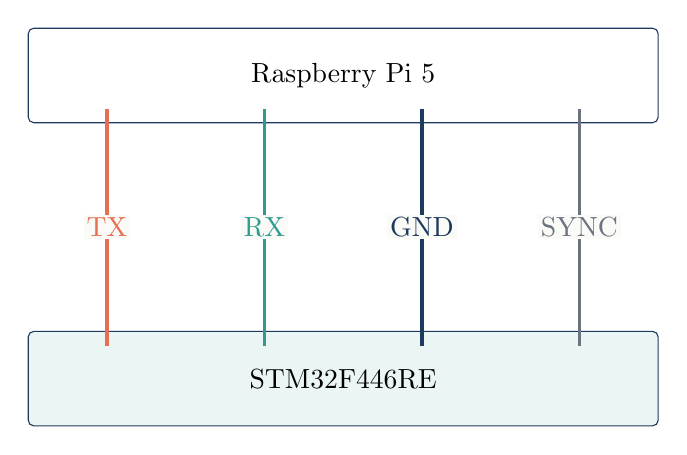
\begin{tikzpicture}[y=.7cm,font=\normalsize,box/.append style={font=\normalsize,minimum height=12mm}]
\node[box,minimum width=80mm] (pi) at (3,1.5) {Raspberry Pi 5};
\node[box,minimum width=80mm,fill=teal!10] (stm) at (3,-4) {STM32F446RE};
\foreach \x/\tag/\col in {0/TX/fault,2/RX/teal,4/GND/navy,6/SYNC/muted}{
\draw[\col,very thick] (\x,.9)--(\x,-3.4);
\node[lbl,font=\normalsize,text=\col] (l\tag) at (\x,-1.25) {\tag};
\draw[\col,thin] (l\tag.south)--(\x,-2.1);}
\end{tikzpicture}}
\csdef{diagramV22}{\wiringdiagram}
\newcommand{\profilesdiagram}{%
\begin{tikzpicture}[font=\normalsize,box/.append style={font=\normalsize,minimum width=20mm,minimum height=12mm}]
\node[box] (p0) at (0,0) {P0};\node[box] (p1) at (0,-2.2) {P1};
\node[box,fill=teal!12] (p2) at (-1.2,-5.3) {P2};\node[box,fill=navy!10] (p3) at (1.2,-5.3) {P3};
\draw[flow] (p0)--node[lbl,right=5pt,font=\normalsize] {Tinh chỉnh} (p1);
\draw[flow] (p1.west)--(-1.2,-2.2)--(p2.north);
\draw[flow] (p1.east)--(1.2,-2.2)--(p3.north);
\node[lbl,font=\normalsize,align=center,anchor=east] at (-1.5,-3.65) {Bộ đệm\\mới nhất};
\node[lbl,font=\normalsize,align=center,anchor=west] at (1.5,-3.65) {Kernel\\PREEMPT\_RT};
\end{tikzpicture}}
\csdef{diagramV12}{\profilesdiagram}
